\subsection{Controlled demonstration}

\paragraph{Setup.}
Does accounting for observational uncertainty change which forecast version wins? I start with a controlled case using the synthetic forecast versions defined in \S5.2, with $y = 50$ and $\sigma_\text{rel} = 0.4$ (the Constructor~3 working default; see \S3 for calibration against the RVI Gumbel model).

\paragraph{Results.}
Classical CRPS ranks the tight version first: its narrow distribution is closer to the step at $y$ at almost every $z$, and the squared-area integrand is smaller. The reformulated metric, computed against a smooth $F_\text{obs}$ constructed via Constructor~3 ($\sigma_\text{rel} = 0.4$), reverses the ranking: the honest version wins. Figure~\ref{fig:reversal} shows the four scores. The reversal is a sign change---which version wins flips---not a numerical artifact. In this baseline case, the reversal is algebraically guaranteed: the Cram\'er distance is an $L^2$ metric, and $\sigma_\text{honest} = \sigma_\text{rel}$ means the honest version's CDF matches $F_\text{obs}$ exactly, which is the minimiser by construction. The substantive question is not \emph{whether} the reversal occurs at the matched parameterisation, but \emph{how far} the honest version can deviate from $F_\text{obs}$ and still beat the overconfident version.

\begin{figure}[h]
    \centering
    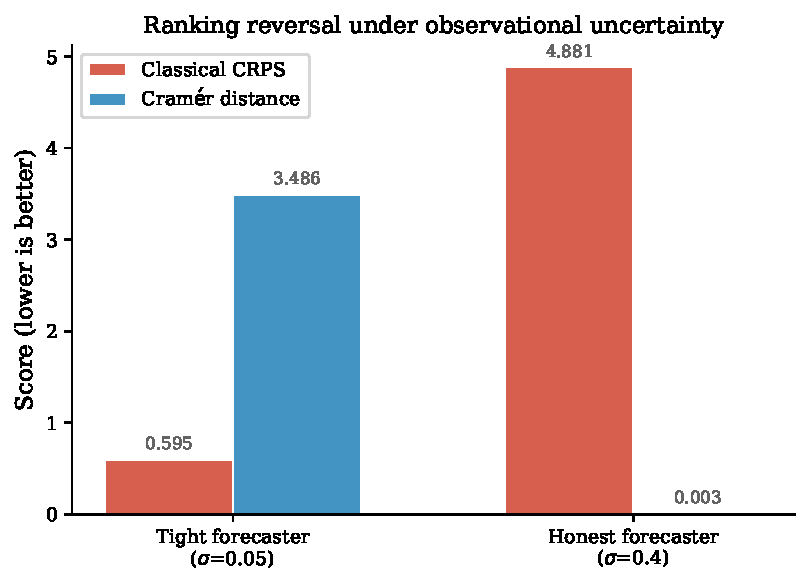
\includegraphics[width=0.7\textwidth]{figures/uncertainty_aware_ranking.pdf}
    \caption{Ranking reversal between two forecast versions on a controlled example. Under classical CRPS the tight (overconfident) version wins; under the Cram\'er-distance reformulation the honest version wins. The reversal is qualitative---the sign of which version is better changes.}
    \label{fig:reversal}
\end{figure}

The reversal does not depend on the honest version exactly matching $F_\text{obs}$: varying $\sigma_\text{honest}$ while holding $\sigma_\text{rel} = 0.4$ fixed, the reversal holds for $\sigma_\text{honest} \in [0.10, \, 0.85]$---the honest version can be $4\times$ too narrow or $2\times$ too wide and still beat the tight version.

\paragraph{When the reversal does not hold.}
The reversal disappears in two parameter regimes: (1)~when observational uncertainty is small ($\sigma_\text{rel} \leq 0.10$), so that $F_\text{obs}$ is close to the classical step function and the reformulated metric behaves like standard CRPS; and (2)~when the honest version is extremely wide ($\sigma_\text{honest} \geq 1.0$), so that its CDF deviates from $F_\text{obs}$ by more than the tight version does. In the first regime, the reformulation is unnecessary---observations are precise enough that classical CRPS is appropriate. In the second, the honest version is not honestly calibrated but genuinely overwide; the metric correctly penalises it. Detailed robustness analysis---including constructor comparison, location-error tolerance, and generalisation across distributional families---is in Appendix~\ref{sec:appendix_demo}.

\subsection{Empirical comparison on UCDP conflict data}

I score both synthetic forecast versions (\S5.2) under classical CRPS and the Cram\'er-distance reformulation with Constructor~3 ($\sigma_\text{rel} = 0.4$) on the UCDP sample described in \S5.1.

Under classical CRPS the tight version wins in 100\% of cell-months---a direct consequence of both versions being centred on $y$ and CRPS's well-known preference for concentration. Under the Cram\'er-distance reformulation, the ranking reverses in 39\% of cell-months overall.\footnote{The reversal rate is sensitive to $\sigma_\text{rel}$: at $\sigma_\text{rel} = 0.3$ it drops to 12.6\%; at $\sigma_\text{rel} = 0.5$ it rises to 67.7\%.} The reversal rate depends sharply on forecast uncertainty: for cells with moderate uncertainty ($\hat{\sigma}_\text{cell} \leq 0.8$; $n = 4{,}716$), the honest version wins in \emph{every} cell-month. For cells with very high uncertainty ($\hat{\sigma}_\text{cell} > 1.0$; $n = 8{,}902$), the honest version is too wide and loses---exactly the regime identified in the controlled demonstration. Figure~\ref{fig:real_data} shows the reversal rate by uncertainty regime and the score-difference distribution.

\begin{figure}[h]
    \centering
    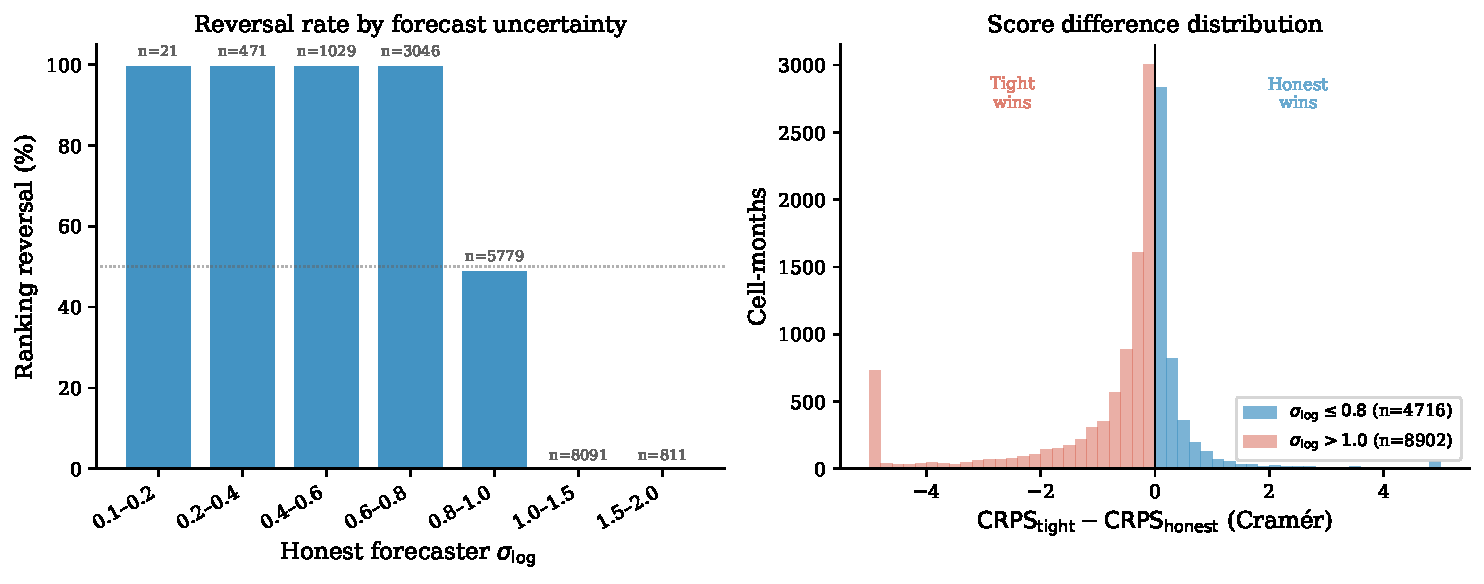
\includegraphics[width=\textwidth]{figures/real_data_comparison.pdf}
    \caption{Ranking reversal on UCDP conflict data (2020--2024, 19{,}397 cell-months). Left: reversal rate under the Cram\'er-distance reformulation as a function of the honest version's log-space uncertainty $\hat{\sigma}_\text{cell}$. The reversal is complete for $\hat{\sigma}_\text{cell} \leq 0.8$ and absent for $\hat{\sigma}_\text{cell} > 1.0$. Right: distribution of score differences; positive values indicate the honest version wins.}
    \label{fig:real_data}
\end{figure}

Among cell-months with genuine UCDP low/best/high bounds, Constructor~1 produces a reversal rate of only 9.9\%---reflecting the fact that UCDP's coding ranges are narrow relative to the true observational uncertainty \citep{vesco2026uncertainty}. Under the RVI Gumbel mixture (Constructor~2), the reversal widens to 80.8\% of cell-months, capturing asymmetric underreporting that the symmetric parametric constructor misses. The Bessac--Naveau conditional-expectation correction \citep{bessac2021forecast} confirms the pattern, with 98.1\% concordance overall. Constructor comparison details and the unit-of-analysis caveat for Constructor~2 are in Appendix~\ref{sec:appendix_demo}.

\paragraph{Per-violence-type analysis.}
Table~\ref{tab:per_type} breaks the comparison down by UCDP violence type. State-based violence ($n = 10{,}760$) shows the lowest RVI reversal rate (79.3\%), consistent with state-based events being better documented and having higher fatality counts on average. Non-state violence ($n = 4{,}363$) shows the highest reversal rate (90.4\%) and is the only type where the RVI Cram\'er distance selects the honest version \emph{on average}---non-state events tend to have smaller counts where underreporting is most severe. One-sided violence ($n = 4{,}003$) falls in between at 84.6\%. A caveat: the per-type differences confound documentation quality with event-size distribution. Non-state events are both less well documented \emph{and} smaller on average; the higher reversal rate could reflect either factor or both. The gradient is nonetheless informative: the Cram\'er-distance reformulation is most consequential for the violence types where observational uncertainty is greatest, and least consequential where data quality is highest.

\begin{table}[h]
    \centering
    \small
    \begin{tabular}{lrrrrrr}
        \toprule
        Violence type & $n$ & Classical & \multicolumn{2}{c}{Parametric} & \multicolumn{2}{c}{RVI Gumbel} \\
        \cmidrule(lr){4-5} \cmidrule(lr){6-7}
         & & tight \% & reversal \% & BN agree \% & reversal \% & BN agree \% \\
        \midrule
        State-based & 10{,}760 & 100\% & 34.8\% & 93.3\% & 79.3\% & 78.2\% \\
        Non-state & 4{,}363 & 100\% & 62.9\% & 94.1\% & 90.4\% & 90.2\% \\
        One-sided & 4{,}003 & 100\% & 43.7\% & 94.3\% & 84.6\% & 84.1\% \\
        \midrule
        All & 19{,}397 & 100\% & 39.0\% & 98.1\%$^\dagger$ & 80.8\% & 98.5\%$^\dagger$ \\
        \bottomrule
    \end{tabular}
    \caption{Ranking reversal rates by UCDP violence type. ``Classical tight~\%'' is the fraction of cell-months where classical CRPS selects the tight version. ``Reversal~\%'' is the fraction where the Cram\'er-distance reformulation reverses the ranking. ``BN agree'' is the Bessac--Naveau concordance---the fraction of cell-months where the Bessac--Naveau conditional-expectation correction agrees with the Cram\'er distance on which version wins---computed separately under each $F_\text{obs}$ constructor (parametric and RVI). The parametric constructor uses $\sigma_\text{rel} = 0.4$; the RVI Gumbel uses the regression coefficients of \citet{vesco2026uncertainty}. Per-type counts do not sum to the pooled total because the historical-statistics join (cells with $\geq 3$ active months) applies per type; 271 cell-months qualify in the pooled analysis but fall below the per-type activity threshold. $^\dagger$Pooled BN concordance uses $M = 2{,}000$ Monte Carlo draws; per-type rows use $M = 200$.}
    \label{tab:per_type}
\end{table}

\subsection{Validation with an operational forecaster}

\paragraph{State-based results.}
I begin with state-based violence, the best-documented type. In the full sample (5{,}372 cell-months), classical CRPS strictly prefers the tight version in only 2.1\% of cell-months (115/5{,}372). A further 36.5\% (1{,}962 cell-months) are ties where the model predicts zero fatalities and both versions are degenerate; the remaining 61.3\% strictly prefer the full MC Dropout version. The dominance of the full MC Dropout version reflects HydraNet's typically large predictive-location errors; when the model misses the target value, wider spread helps under classical CRPS simply by placing more mass near the target.

The interesting regime is the 589 cell-months (11.0\%) where the model's prediction falls within a factor of two of the actual---where predictive-location error is moderate and the spread dimension becomes consequential. In this subset, classical CRPS selects the tight version in 115 cell-months (19.5\%). The Cram\'er-distance reformulation (Constructor~3, $\sigma_\text{rel} = 0.4$) reverses 114 of these 115 cases (99.1\%), selecting the full MC Dropout version instead. Under the RVI Gumbel constructor (Constructor~2), the reversal rate is 110/115 (95.7\%). The cell-months that resist reversal are high-fatality cases where the full MC Dropout version's spread genuinely exceeds $F_\text{obs}$---the Cram\'er distance penalises overwide uncertainty, exactly as in the synthetic demonstration.

\paragraph{Per-type analysis.}
Table~\ref{tab:hydranet_reversal} extends the analysis to all three violence types. The reversal pattern holds across types: in the factor-of-two subset, the parametric constructor reverses $\geq 94\%$ and the RVI constructor reverses $\geq 96\%$ of classical tight-version preferences. One-sided violence shows 100\% reversal under both constructors, consistent with one-sided events carrying the highest observational uncertainty (small counts, limited documentation).

\begin{table}[h]
    \centering
    \small
    \begin{tabular}{lrrrrr}
        \toprule
        Violence type & $n$ & Classical & \multicolumn{2}{c}{Reversal rate} \\
        \cmidrule(lr){4-5}
         & & tight \% & Parametric & RVI Gumbel \\
        \midrule
        State-based & 589 & 19.5\% & 99.1\% & 95.7\% \\
        Non-state & 188 & 28.7\% & 94.4\% & 98.1\% \\
        One-sided & 148 & 24.3\% & 100.0\% & 100.0\% \\
        \bottomrule
    \end{tabular}
    \caption{HydraNet ranking reversal in the factor-of-two subset by violence type. $n$ is the number of cell-months where the model's predictive mean falls within a factor of two of the reported value. ``Classical tight~\%'' is the fraction where classical CRPS selects the tight version. ``Reversal rate'' is the fraction of those classical tight selections that the Cram\'er-distance reformulation reverses. The parametric constructor uses $\sigma_\text{rel} = 0.4$; the RVI Gumbel uses the regression coefficients of \citet{vesco2026uncertainty}.}
    \label{tab:hydranet_reversal}
\end{table}

\subsection{Sensitivity to $F_\text{obs}$ mis-specification}

Could the metric's behaviour under a mis-specified $F_\text{obs}$ be worse than classical CRPS with no $F_\text{obs}$ at all? I quantify this by running the stochastic consistency check from \S4 (details in Appendix~\ref{sec:appendix_consistency}) under deliberate mis-specification. The true data-generating distribution is $\text{LogNormal}(\mu = 1.0, \sigma = 0.3)$; I construct $F_\text{obs}$ using $\sigma_\text{rel}$ values ranging from $0.1$ to $1.0$ and ask where the expected Cram\'er distance is minimised.

Table~\ref{tab:misspec} shows the results. When $\sigma_\text{rel}$ matches the true $\sigma$ (ratio 1.0$\times$), the argmin falls exactly on $\mu_\text{true}$. Moderate overestimation (up to 2$\times$) shifts the argmin by at most one grid step ($+0.05$). Severe overestimation (3.3$\times$) shifts it by $+0.15$---meaningful but bounded. Underestimation produces no detectable bias in this sweep. For this log-normal DGP, the bias is monotonic in the mis-specification ratio; whether monotonicity holds across distributional families is untested, but the practical implication---a practitioner can bound the bias by bounding the mis-specification---applies whenever the relationship is monotone.

The asymmetry has a structural explanation. When $\sigma_\text{rel}$ is underestimated, $F_\text{obs}$ approaches the degenerate step function at $y$, and the Cram\'er distance reduces to classical CRPS---which is proper, so the location argmin remains at $\mu_\text{true}$. When $\sigma_\text{rel}$ is overestimated, $F_\text{obs}$ is wider than the true observation noise; the log-normal right-skew of the widened $F_\text{obs}$ shifts the $L^2$-minimising location upward, producing positive bias. The same mechanism explains the scale-consistency convolution effect discussed in \S4 and Appendix~\ref{sec:appendix_consistency}: the metric measures distance from the observable distribution, which inherits the observation noise.

A formal characterisation of this bias is an open problem.

\begin{table}[h]
    \centering
    \small
    \begin{tabular}{rrrr}
        \toprule
        $\sigma_\text{rel}$ & Ratio ($\sigma_\text{rel} / \sigma_\text{true}$) & Argmin $\hat{\mu}$ & Location bias ($\hat{\mu} - \mu_\text{true}$) \\
        \midrule
        0.1 & 0.3$\times$ & 1.000 & 0.000 \\
        0.2 & 0.7$\times$ & 1.000 & 0.000 \\
        0.3 & 1.0$\times$ & 1.000 & 0.000 \\
        0.4 & 1.3$\times$ & 1.050 & $+$0.050 \\
        0.6 & 2.0$\times$ & 1.050 & $+$0.050 \\
        0.8 & 2.7$\times$ & 1.100 & $+$0.100 \\
        1.0 & 3.3$\times$ & 1.150 & $+$0.150 \\
        \bottomrule
    \end{tabular}
    \caption{Argmin bias under mis-specified $F_\text{obs}$. The true DGP is $\text{LogNormal}(1.0, 0.3)$; $F_\text{obs}$ uses varying $\sigma_\text{rel}$. Monte Carlo expectation over 500 draws. Grid step $= 0.05$.}
    \label{tab:misspec}
\end{table}
